\documentclass[tikz,border=10pt]{standalone}
\usetikzlibrary{angles}

\begin{document}

% Q1
\begin{tikzpicture}[scale=1, transform shape]
    % Define the points of the cube
    \coordinate (A) at (0,0);
    \coordinate (B) at (3,0);
    \coordinate (C) at (0,4);

    % Draw the triangle
    \draw (A) -- (B) -- (C) -- cycle; 

    % Draw the angles
    \draw pic[draw, angle radius=2.5mm] {right angle=C--A--B};

    % Place the labels with smaller font size
    \node at (A) [left,font=\small] {A};
    \node at (B) [right,font=\small] {B};
    \node at (C) [above left,font=\small] {C};

    % Place the labels with smaller font size
    \draw (A) -- (B) node[midway, below] {8cm};
    \draw (A) -- (C) node[midway, left] {6cm};
    
\end{tikzpicture}

% Q2
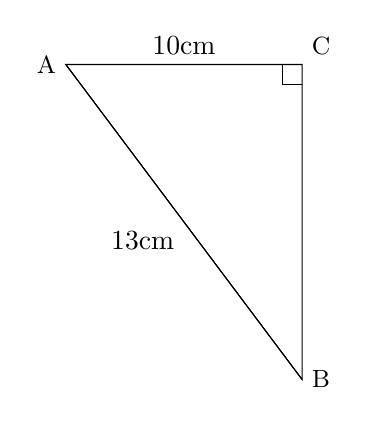
\begin{tikzpicture}[scale=1, transform shape]
    % Define the points of the cube
    \coordinate (A) at (0,4);
    \coordinate (B) at (3,0);
    \coordinate (C) at (3,4);

    % Draw the triangle
    \draw (A) -- (B) -- (C) -- cycle; 

    % Draw the angles
    \draw pic[draw, angle radius=2.5mm] {right angle=A--C--B};

    % Place the labels with smaller font size
    \node at (A) [left,font=\small] {A};
    \node at (B) [right,font=\small] {B};
    \node at (C) [above right,font=\small] {C};

    % Place the labels with smaller font size
    \draw (A) -- (B) node[midway, below left] {13cm};
    \draw (A) -- (C) node[midway, above] {10cm};

\end{tikzpicture}

% Q3
\begin{tikzpicture}[scale=1, transform shape]
    % Define the points of the cube
    \coordinate (A) at (0,4);
    \coordinate (B) at (0,0);
    \coordinate (C) at (3,4);

    % Draw the triangle
    \draw (A) -- (B) -- (C) -- cycle; 

    % Draw the angles
    \draw pic[draw, angle radius=2.5mm] {right angle=C--A--B};

    % Place the labels with smaller font size
    \node at (A) [left,font=\small] {A};
    \node at (B) [below left,font=\small] {B};
    \node at (C) [right,font=\small] {C};

    % Place the labels with smaller font size
    \draw (A) -- (B) node[midway, below left] {9.3cm};
    \draw (A) -- (C) node[midway, above] {4.2m};
    
\end{tikzpicture}

% Q4
\begin{tikzpicture}[scale=1, transform shape]
    % Define the points of the cube
    \coordinate (A) at (0,0);
    \coordinate (B) at (0,5);
    \coordinate (C) at (4,3);
    \coordinate (D) at (4,0);

    % Draw the triangle
    \draw (A) -- (B) -- (C) -- (D) -- cycle; 

    % Draw the angles
    \draw pic[draw, angle radius=2.5mm] {right angle=B--A--D};
    \draw pic[draw, angle radius=2.5mm] {right angle=A--D--C};

    % Place the labels with smaller font size
    \node at (A) [below left,font=\small] {A};
    \node at (B) [above left,font=\small] {B};
    \node at (C) [right,font=\small] {C};
    \node at (D) [below right,font=\small] {D};

    % Place the labels with smaller font size
    \draw (A) -- (B) node[midway, left] {9cm};
    \draw (B) -- (C) node[midway, above right] {10cm};
    \draw (D) -- (C) node[midway, right] {5cm};
    
\end{tikzpicture}

% Q5
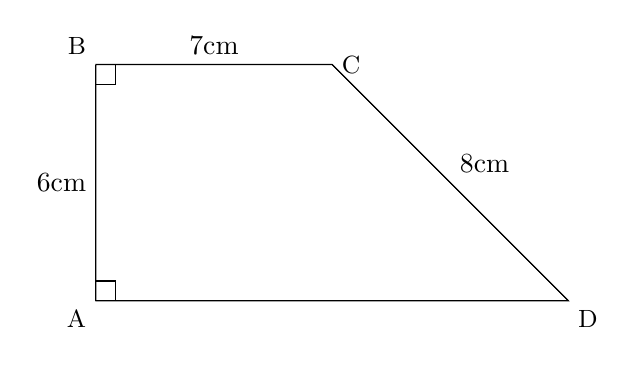
\begin{tikzpicture}[scale=1, transform shape]
    % Define the points of the cube
    \coordinate (A) at (0,0);
    \coordinate (B) at (0,3);
    \coordinate (C) at (3,3);
    \coordinate (D) at (6,0);

    % Draw the triangle
    \draw (A) -- (B) -- (C) -- (D) -- cycle; 

    % Draw the angles
    \draw pic[draw, angle radius=2.5mm] {right angle=B--A--D};
    \draw pic[draw, angle radius=2.5mm] {right angle=C--B--A};

    % Place the labels with smaller font size
    \node at (A) [below left,font=\small] {A};
    \node at (B) [above left,font=\small] {B};
    \node at (C) [right,font=\small] {C};
    \node at (D) [below right,font=\small] {D};

    % Place the labels with smaller font size
    \draw (A) -- (B) node[midway, left] {6cm};
    \draw (B) -- (C) node[midway, above] {7cm};
    \draw (D) -- (C) node[midway, above right] {8cm};
    
\end{tikzpicture}

% Q6
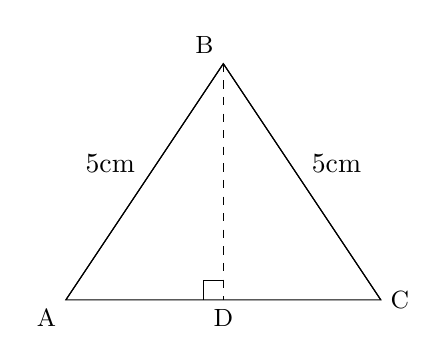
\begin{tikzpicture}[scale=1, transform shape]
    % Define the points of the cube
    \coordinate (A) at (0,0);
    \coordinate (B) at (2,3);
    \coordinate (C) at (4,0);
    \coordinate (D) at (2,0);

    % Draw the triangle
    \draw (A) -- (B) -- (C) -- cycle; 
    \draw[dashed] (B) -- (D);

    % Draw the angles
    \draw pic[draw, angle radius=2.5mm] {right angle=A--D--B};

    % Place the labels with smaller font size
    \node at (A) [below left,font=\small] {A};
    \node at (B) [above left,font=\small] {B};
    \node at (C) [right,font=\small] {C};
    \node at (D) [below,font=\small] {D};

    % Place the labels with smaller font size
    \draw (A) -- (B) node[midway, above left] {5cm};
    \draw (B) -- (C) node[midway, above right] {5cm};
    
\end{tikzpicture}

% Q7
\begin{tikzpicture}[scale=1, transform shape]
    % Define the points of the cube
    \coordinate (A) at (0,4);
    \coordinate (B) at (3,0);
    \coordinate (C) at (3,4);
    \coordinate (D) at (10,4);

    % Draw the triangle
    \draw (A) -- (B) -- (C) -- cycle; 
    \draw (B) -- (C) -- (D) -- cycle;

    % Draw the angles
    \draw pic[draw, angle radius=2.5mm] {right angle=A--C--B};

    % Place the labels with smaller font size
    \node at (A) [left,font=\small] {A};
    \node at (B) [below,font=\small] {B};
    \node at (C) [above,font=\small] {C};
    \node at (D) [right,font=\small] {D};

    % Place the labels with smaller font size
    \draw (A) -- (B) node[midway, below left] {9cm};
    \draw (A) -- (C) node[midway, above] {5cm};
    \draw (B) -- (D) node[midway, below right] {13cm};

\end{tikzpicture}

\end{document}
